\section{Gaussian Mixture Models}

\subsection{Multinomial Distribution}
$$P(X|\boldsymbol{\mu}) = \prod_{n} \prod_k \mu_k^{x_{nk}} = \prod_k\mu_k^{\sum_n x_{nk}}.$$
How to determine the MLE solution of $\boldsymbol{\mu}?$ \ie maximize$P(X|\boldsymbol{\mu})$ subject to $\mu_k\geq 0$ and $ \sum_k \mu_k = 1$. We can use the Lagrange method. 

\begin{align*}
	&\mathcal{L} = \sum_k\sum_nx_{nk}\ln \mu_k +\lambda(\sum_k\mu_k-1)\\ 
	&\frac{\partial \mathcal{L}}{\partial \mu_k} = \frac{\sum_nx_{nk}}{\mu_k}+\lambda. \\
	& \mu_k^{\textrm{ML}} = \frac{m_k}{N},
\end{align*}
where $m_k = \sum_n x_{nk}.$ We can consider the joint distribution of the quantities $m_1, \dots, m_K$, conditioned on the parameters $\boldsymbol{\mu}$ and on the total number $N$ observations: 
$$\textrm{Mult}(m_1, \dots, m_K|\boldsymbol{\mu}, N) = \binom{N}{m_1, \dots, m_K} = \frac{N!}{m_1!,\dots, m_K!}.$$
Note that the variables $m_k$ are subject to the constraint
$$\sum_k m_k = N.$$


\subsection{Multivariate Gaussian Distribution}
\begin{align*}
	\mathcal{N}(x|\mu,\sigma^2) = \frac{1}{\sqrt{2\pi\sigma^2}}\exp\bigg(-\frac{1}{2\sigma^2}(x-\mu)^2\bigg)
\end{align*}
For a $D$-dimensional vector $\mathbf{x}$, 
\begin{align*}
	\mathcal{N}(\mathbf{x}|\boldsymbol{\mu},\boldsymbol{\Sigma}) &= \frac{1}{(2\pi)^{D/2}|\boldsymbol{\Sigma}|^{1/2}}\exp\bigg(-\frac{1}{2}(\mathbf{x}-\boldsymbol{\mu})^T\boldsymbol{\Sigma}^{-1}(\mathbf{x}-\boldsymbol{\mu})\bigg)\\
	\ln\mathcal{N}(\mathbf{x}|\boldsymbol{\mu},\boldsymbol{\Sigma}) &= -\frac{1}{2}\ln|\boldsymbol{\Sigma}|-\frac{1}{2}(\mathbf{x}-\boldsymbol{\mu})^T\boldsymbol{\Sigma}^{-1}(\mathbf{x}-\boldsymbol{\mu})+C.
\end{align*}
Note that the functional dependence of the Gaussian on $\mathbf{x}$ is through the quadratic form: 
$$\Delta^2 = (\mathbf{x}-\boldsymbol{\mu})^T\boldsymbol{\Sigma}^{-1}(\mathbf{x}-\boldsymbol{\mu}).$$
The quantity $\Delta$ is called the \textit{Mahalanobis distance} from $\boldsymbol{\mu}$ to $\mathbf{x}$ and reduces to the Euclidean distance when $\boldsymbol{\Sigma}$ is the identity matrix.

Also,by using i.i.d. condition of a dataset, we can also express as follows:
\begin{align*}
	\ln\mathcal{N}(\mathbf{X}|\boldsymbol{\mu},\boldsymbol{\Sigma}) &= -\frac{N}{2}\ln|\boldsymbol{\Sigma}|-\frac{1}{2}\sum_n(\mathbf{x}_n-\boldsymbol{\mu})^T\boldsymbol{\Sigma}^{-1}(\mathbf{x}_n-\boldsymbol{\mu})+C
\end{align*}








\subsection{Gaussian Mixture Models}


K-means clustering is a hard-clustering, but in some cases soft-clustering provides a better model in practice. Gaussian mixture model assumes a simple \textbf{linear superposition} of Gaussian components, aimed at providing a richer class of density models than the single Gaussian. Let's consider a single sample case and it can be expressed as follows:
$$p(\mathbf{x})= \sum_{k=1}^{K}\pi_k\mathcal{N}(\mathbf{x}|\boldsymbol{\mu_k}, \boldsymbol{\Sigma}_k)$$
Let us introduce a $K$-dimensional binary random variable $\mathbf{z}$ having a 1-of-$K$ representation in which a particular element $z_k$ is equal to 1 and all other elements are 0. I will explain more about $\mathbf{z}$ later. It satisfied the following properties:
\begin{itemize}
	\item $z_k\in\{0,1\}$
	\item $\sum_kz_k=1$
\end{itemize}
The marginal distribution over $\mathbf{z}$ is specified in terms of the mixing coefficients $\pi_k$, such that 
$$p(z_k=1) = \pi_k$$
, where the mixing coefficients must satisfy
$$0\leq\pi_k\leq1$$
and 
$$\sum_{k=1}^{K}\pi_k = 1 $$
in order to be valid probabilities. We can also write pdf of $\mathbf{z}$ in a product of mixing coefficient because it is a 1-of-$K$ representaion.
$$p(\mathbf{z}) = \prod_{k=1}^{K}\pi_k^{z_k} = \pi_k \because z_k\in\{
0,1\}$$
Similarly, the conditional distribution of $\mathbf{x}$ given a particular $\mathbf{z}$ can be modeled to be a Gaussian distribution.
\begin{equation*}
p(\mathbf{x}|z_k=1) = \mathcal{N}(\mathbf{x}|\boldsymbol{\mu}_k, \boldsymbol{\Sigma}_k) 
\end{equation*}
Also can be represented in the form 
\begin{align*}
p(\mathbf{x}|\mathbf{z}) &= \prod_{k=1}^{K}\mathcal{N}(\mathbf{x}|\boldsymbol{\mu}_k, \boldsymbol{\Sigma}_k)^{z_k}\\
& = \mathcal{N}(\mathbf{x}|\boldsymbol{\mu}_k, \boldsymbol{\Sigma}_k) \because z_k\in\{
0,1\}
\end{align*}
Finally, marginal data distribution can be obtrained by summing the joint distribution over all possible states of $\mathbf{z}$ to give
\begin{align*}
	p(\mathbf{x}) &  = \sum_{\mathbf{z}} p(\mathbf{x},\mathbf{z})\\
	& = \sum_{\mathbf{z}} p(\mathbf{z})p(\mathbf{x}|\mathbf{z})= \sum_{z_1,...,z_K} p(z_1,...,z_K)p(\mathbf{x}|z_1,...,z_K)\\
	& = \sum_{k=1}^{K}\pi_k \mathcal{N}(\mathbf{x}|\boldsymbol{\mu}_k, \boldsymbol{\Sigma}_k) 
\end{align*}
Note that for every observed data point $\mathbf{x}_n$ there is a corresponding latent variable $\mathbf{z}_n$, which \textbf{indicates the membership of} $\mathbf{x}_n$. This can be represented as in Fig. \ref{fig:gmm}.

\begin{figure}[h]
	\begin{center}			
		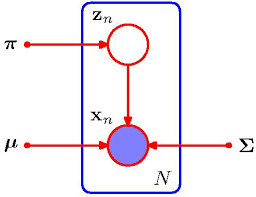
\includegraphics[scale=0.4]{./images/generative/gmm.png}
	\end{center}
	\caption{Graphical representation of GMM model. The GMM models a joint distribution $p(\mathbf{x}, \mathbf{z})$ in terms of a marginal distribution $p(\mathbf{z})$ and conditional distribution $p(\mathbf{x}|\mathbf{z})$ to model $p(\mathbf{x})$. Each $\mathbf{x}_n$ is coupled with $\mathbf{z}_n$}
	\label{fig:gmm}
\end{figure}
Now we can work with the joint distribution $p(\mathbf{x,z})$ instead of the marginal distribution $p(\mathbf{x})$, which is hard to estimate directly as explained in \Cref{sec:intro_motivation}. 

Another quantity which plays a central role is the conditional proability of $\mathbf{z}$ given $\mathbf{x}$, $p(z_k=1|\mathbf{x})$. 
\begin{itemize}
\item $p(z_k=1) = \pi_k$ can be viewed as a prior of $z_k=1$
\item $\gamma(z_k)$: assignment probability or responsibility. This represents the probability of assignment of a sample.  This quantity will be updated through the Bayes Theorem.
\item[] $\rightarrow$  A simple explanation is that \textbf{this is the classification result} of $\mathbf{x}_n$.
\end{itemize}
\begin{align*}
\gamma(z_k) \equiv p(z_k=1|\mathbf{x}) & \equiv \frac{p(z_k=1)p(\mathbf{x}|z_k=1)}{\sum_{j=1}^{K}p(z_j=1)p(\mathbf{x}|z_j=1)} \\
& = \frac{\pi_k\mathcal{N}(\mathbf{x}|\boldsymbol{\mu}_k, \boldsymbol{\Sigma}_k)}{\sum_{j=1}^{K} \pi_j\mathcal{N}(\mathbf{x}|\boldsymbol{\mu}_j, \boldsymbol{\Sigma}_j)}
\end{align*}

\subsection{Maximum Likelihood}
Suppose we have a data set of observations $\mathbf{X}=\{\mathbf{x}_1,...,\mathbf{x}_n\}^{T}\in\mathbb{R}^{N\times D}$ and we want to model the data distribution $p(\mathbf{X})$ using GMM. If we assume an \textrm{i.i.d.} data set, it can be expressed as follows: 
\begin{align*}
p(\mathbf{X}|\boldsymbol{\pi},\boldsymbol{\mu},\boldsymbol{\Sigma}) &=\prod_{n=1}^{N}\Bigg(\sum_{k=1}^{K}\pi_k\mathcal{N}(\mathbf{x}_n|\boldsymbol{\mu}_k, \boldsymbol{\Sigma}_k)\Bigg)\\
\end{align*}
then its \textbf{loglikelihood function for GMM} is given by:
\begin{align*}
\ln p(\mathbf{X}|\boldsymbol{\pi},\boldsymbol{\mu},\boldsymbol{\Sigma}) &= \sum_{n=1}^{N}\ln \Bigg(\sum_{k=1}^{K}\pi_k\mathcal{N}(\mathbf{x}_n|\boldsymbol{\mu}_k, \boldsymbol{\Sigma}_k)\Bigg)
\end{align*}

%In a single dimension case, 
%\begin{align*}
%	\ln p(x, \pi, \mu, \sigma) & =\sum_{n=1}^{N}\ln \sum_{k=1}^{K}\pi_k \frac{1}{\sigma_k \sqrt{2\pi_k}}\exp\Big(-\frac{1}{2}\Big(\frac{x_n-\mu_k}{\sigma_k}\Big)^2\Big)\\
%	\frac{\partial }{\partial \mu_k}\ln p(x, \pi, \mu, \sigma) & =\sum_{n=1}^{N} \frac{\pi_k \frac{1}{\sigma_k \sqrt{2\pi}}\exp\Big(-\frac{1}{2}\Big(\frac{x_n-\mu_k}{\sigma_k}\Big)^2\Big) \frac{x_n-\mu_k}{\sigma_k^2}}{\sum_{k=1}^{K}\pi_k \frac{1}{\sigma_k \sqrt{2\pi}}\exp\Big(-\frac{1}{2}\Big(\frac{x_n-\mu_k}{\sigma_k}\Big)^2\Big)}\\
%	& =\sum_{n=1}^{N} \underbrace{\frac{\pi_k \mathcal{N}(x_n|\mu_k, \sigma_k) }{\sum_{k=1}^{K}\pi_k \mathcal{N}(x_n|\mu_k, \sigma_k)}}_{=\gamma(z_{nk})}\frac{x_n-\mu_k}{\sigma_k^2}\\
%	\mu_k &=\frac{1}{N_k}\sum_{n=1}^{N} \gamma(z_{nk}) x_n,
%\end{align*}
%where 
%$N_k = \sum_{n=1}^{N} \gamma(z_{nk})$. $N_k$ can be interpreted as the effective number of points assigned to cluster $k$. 

How to solve this MLE? While a gradient-based optimization is possible, we consider the iterative \textit{Expectation Maximization} algorithm.

Before, maximizing the likelihood, it is worth to emphasize two issues in GMM: (i) \textit{singularities} and (ii) \textit{identifiability}.

%\subsection{Singularity and Identifiability}
\paragraph{Singularity}
% Suppose that one of the components of the mixture model, let us say the $j$-th component, has its mean $\mathbf{\mu}_j$ exactly equal to one of the data points so that $\mathbf{\mu}_j=\mathbf{x}_n$ for some value of $n$. This data point will then contributes a term in the likelihood function of the form 
% $$\mathcal{N}(\mathbf{x}_n, \sigma_j^2\mathbf{I}) = \frac{1}{(2\pi)^{1/2}} \frac{1}{\sigma_j}$$
% If we consider the limit $\sigma_j \to 0$, then we see that this term goes to infinity and so the log likelihood function will also go to infinity. Thus the maximization of the log likelihood function will also go to infinity. Thus the maximization of the log likelihood function is not a well posed problem because such sigularities will walways be present and will occur whenever one of the Gaussian components collapses onto a specific data point. 

Before discussing how to maximize this function, it is worth emphasizing that there is a significant problem associated with the maximum likelihood framework applied to Gaussian mixture models, due to the presence of singularities. For simplicity, consider a Gaussian mixture whose components have covariance matrices given by $\Sigma_k = \sigma^2_kI$, where $I$ is the unit matrix, although the conclusions will hold for general covariance matrices. Suppose that one of the components of the mixture model, let us say the $j$-th component, has its mean $\boldsymbol{\mu}_j$ exactly equal to one of the data points so that $\boldsymbol{\mu}_j = \mathbf{x}_n$ for some value of $n$. This data point will then contribute a term in the likelihood function of the form
\begin{align*}
	\mathcal{N}(\mathbf{x}_n|\mathbf{x}_n, \sigma^2_jI) = \frac{1}{\sqrt{2\pi}\sigma_j}
\end{align*}
If we consider the limit $\sigma_j \to 0$, then we see that this term goes to infinity and so the log likelihood function will also go to infinity. Thus the maximization of the log likelihood function is not a well posed problem because such singularities will always be present and will occur whenever one of the Gaussian components `collapses' onto a specific data point. Recall that this problem did not arise in the case of a single Gaussian distribution as the variance can not be zero (recall the definition of variance). 


\paragraph{Identifiability}
A further issue in finding MLE based solutions arises from the fact that for any given maximum likelihood solution, a $K$-component mixture will have a total ok $K!$ equivalent solutions corrsponding to the $K!$ ways of assigning $K$ sets of parameters to $K$ components. In other words, for any given point in the space of parameter values there will be a further $K!-1$ additional points all of which give rise to exactly the same distribution. 

\subsection{Expectation Maximization for GMM}

The goal of Expectation Maximization (EM) is to find maximum likelihood solutions for models having latent variables 
\begin{itemize}
	\item Suppose that it is hard to optimize $p(\mathbf{X}|\boldsymbol{\theta})$ directly.
	\item However, it is easier to optimize the complete-data likelihood function $p(\mathbf{X}, \mathbf{Z}|\boldsymbol{\theta})$ 
	\item In this case, we can use \textbf{EM algorithm}. EM algorithm is a general technique for finding maximum likelihood solutions for latent variable models. 
\end{itemize}
Let us begin by writing down the conditions that must be satisfied at a maximum of the likelihood function. Setting the derivatives of $\ln p(\mathbf{X}|\boldsymbol{\pi},\boldsymbol{\mu},\boldsymbol{\Sigma})$  with respect to the means $\boldsymbol{\mu}_k$ of the Gaussian components to zero, we obtain
\begin{align*}
	0 = -\sum_{n=1}^N\frac{\pi_k\mathcal{N}(\mathbf{x}|\boldsymbol{\mu}_k, \boldsymbol{\Sigma}_k)}{\sum_{j=1}^{K} \pi_j\mathcal{N}(\mathbf{x}|\boldsymbol{\mu}_j, \boldsymbol{\Sigma}_j)}\boldsymbol{\Sigma}_k(\mathbf{x}_n-\boldsymbol{\mu}_k)
\end{align*}
Multiplying by $\boldsymbol{\Sigma}_k^{-1}$ (which we assume to be non-singular) and rearranging we obtain
\begin{align*}
	\boldsymbol{\mu}_k = \frac{1}{N_k}\sum_{n=1}^{N}\gamma(z_{nk})\mathbf{x}_n, 
\end{align*}
where we have defined
\begin{align*}
	N_k = \sum_{n=1}^{N}\gamma(z_{nk}).
\end{align*}
We can interpret $N_k$ as the effective number of points assigned to cluster $k$. We can obtain the MLE solutions for other variables similarly.
\begin{algorithm}
	Initialize the means $\boldsymbol{\mu}_k$, covariances $\boldsymbol{\Sigma}_k$ and mixing coefficients $\pi_k$ and evaluate the initial value of the log likelihood.\\
	\For{n}{
		E step: evaluate the responsibilities of $\mathbf{x}_n$ based on the current parameter values with the given parameters
		$$ \gamma(z_{nk})= p(z_k=1|\mathbf{x}_n) =  \frac{\pi_k\mathcal{N}(\mathbf{x}_n|\boldsymbol{\mu}_k, \boldsymbol{\Sigma}_k)}{\sum_{j=1}^{K} \pi_j\mathcal{N}(\mathbf{x}_n|\boldsymbol{\mu}_j, \boldsymbol{\Sigma}_j)}$$\\
		where $z_{nk}$ denote the $k$-th component of $\mathbf{z}_n$\\
		M step: maximize expectation
		\begin{itemize}
			\item $\boldsymbol{\mu}_k^{\textrm{new}} = \frac{1}{N_k}\sum_{n=1}^{N}\gamma(z_{nk})\mathbf{x}_n$
			\item $\boldsymbol{\Sigma}_k^{\textrm{new}} = \frac{1}{N_k}\sum_{n=1}^{N}\gamma(z_{nk})(\mathbf{x}_n-\boldsymbol{\mu}_k^{\textrm{new}})(\mathbf{x}_n-\boldsymbol{\mu}_k^{\textrm{new}})^T$
			\item $\pi_k^{\textrm{new}} = p(z_k=1) = \frac{N_k}{N}$
		\end{itemize}
	Evaluate the log likelihood to check for convergence of parameters
	$$\textrm{ln}p(\mathbf{X}|\boldsymbol{\pi},\boldsymbol{\mu},\boldsymbol{\Sigma}) = \sum_{n=1}^{N}\textrm{ln}\Bigg(\sum_{k=1}^{K}\pi_k\mathcal{N}(\mathbf{x}_n|\boldsymbol{\mu}_k, \boldsymbol{\Sigma}_k)\Bigg)$$
	}
	\caption{EM algorithm for GMM}
\end{algorithm}
	\begin{figure}[h]
	\begin{center}
		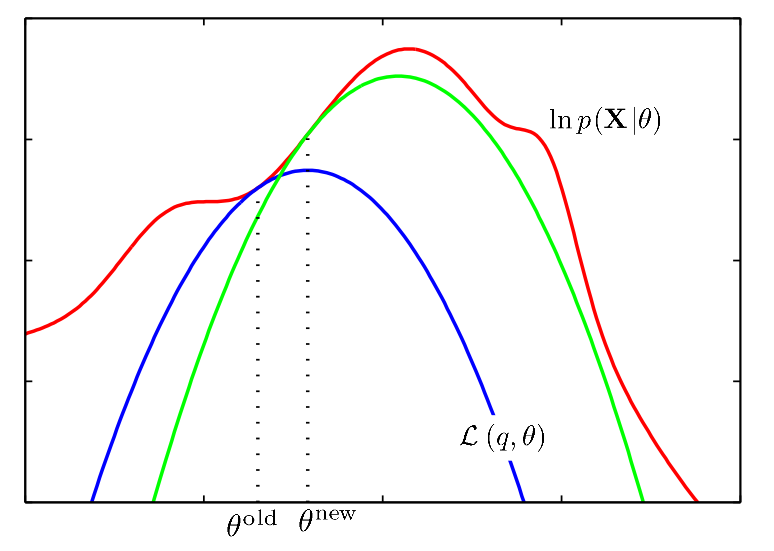
\includegraphics[scale=0.3]{./images/generative/em_update.png}
	\end{center}
	\caption{M-step of EM algorithm}
	\label{fig:em2}
\end{figure}

\section{Alternative View of EM}
The goal of the EM algorithm is to find maximum likelihood (loglikelihood) solutions for models having latent variables.
$$\ln p(X|\theta) = ln\sum_Z p(X,Z|\theta).$$
We are not given the complete data set ${X, Z}$, but only the incomplete data $X$. Our state of knowledge of the values of the latent variables
in $Z$ is given only by the posterior distribution $p(Z|X, \theta)$. Because we cannot use the complete-data log likelihood, we consider instead its expected value under the posterior distribution of the latent variable, which corresponds (as we shall see) to the E step of the EM algorithm.

In the subsequent M step, we maximize this expectation. If the current estimate for the parameters is denoted $\theta_{old}$, then a pair of successive E and M steps gives rise to a revised estimate $\theta^{new}$.

The algorithm is initialized by choosing some starting value for the parameters $\theta_0$. The use of the expectation may seem somewhat arbitrary.

In the E step, we use the current parameter values $\theta^{old}$ to find the posterior distribution of the latent variables given by $p(Z|X, \theta^{old})$. We then use this posterior distribution to find the expectation of the complete-data log likelihood evaluated for some general parameter value $\theta$. This expectation, denoted $Q(\theta, \theta^{old})$, is given by 
$$Q(\theta, \theta^{old}) = \sum_Z p(Z|X, \theta^{old})\ln p(X,Z|\theta).$$
In the M step, we determine the revised parameter estimate $\theta^{new}$ by maximizing this function
$$\theta^{new}=\argmax Q(\theta, \theta^{old}).$$


\begin{algorithm}
The goal is to maximize the likelihood function $p(X|\theta)$ with respect to $\theta$ given a joint distribution $p(X, Z|\theta)$.\\
1. Init $\theta^{old}$\\
2. E-Step: evaluate $p(Z|X, \theta^{old})$ \\
3. M-Step: evaluate $\theta^{new}$ given by 
$$\theta^{new} = \argmax Q(\theta, \theta^{old}),$$
where
$$Q(\theta, \theta^{old}) = \sum_Z p(Z|X, \theta^{old})\ln p(X,Z|\theta).$$
4. Check for convergence of either the log likelihood or the parameter values. If the convergence criterion is not satisfied, then let
$$\theta^{old}\leftarrow \theta^{new}.$$
Return to the step 2. 
\caption{General EM algorithm}
\end{algorithm}

